\documentclass{beamer}\usetheme{boxes}

\usepackage{amsmath,hyperref}

\newcommand{\Mp}{\ensuremath{{M_{+}}}}
\newcommand{\barMp}{\ensuremath{\overline{\Mp}}}
\newcommand{\Dt}{\ensuremath{\Delta t}}
\newcommand{\tM}[1]{\ensuremath{\tilde{M}(#1)}}
\newcommand{\tMt}{\tM{\tau}}
\newcommand{\tMB}{\ensuremath{{\tilde{M}_B}}}
\newcommand{\tE}[1]{\ensuremath{{\tilde{E}(#1)}}}
\newcommand{\tEt}{\tE{\tau}}

\newcommand{\bskip}{\\~\\}
\usepackage{Sweave}
\begin{document}
\Sconcordance{concordance:moz-model-pres.tex:moz-model-pres.Rnw:%
1 14 1 1 0 25 1 1 13 1 2 267 1}

\title{Slightly Less Simple Mosquito Modeling}
\author[Pearson]{Carl~A.~B.~Pearson}
\institute[University of Florida]{
Emerging Pathogens Institute, University of Florida
}
\frame{\titlepage}

\frame{
\frametitle{What's this talk really about?}
\begin{itemize}
\item finding low-hanging fruit,
\item expression with models,
\item simple analytical approaches,
\item a little dimensional analysis,
\item how to connect those with experiments and get higher up the tree, and
\item a little about work habits and tools
\end{itemize}
% I'm going to talk about a project I'm just starting, so the associated science / analysis probably seems simple.  That's a surprisingly good place to start -- small, with some ideas in the back of your mind of where to go from there.  This is kind of the modeling complement to Ray's point about looking at low moments in your data, Fourier components, etc - figure out what the basic views are telling you, and use that to find out where to go.
}

\frame{
\frametitle{A Not Atypical Model of Vector Population}
\begin{figure}
\begin{center}
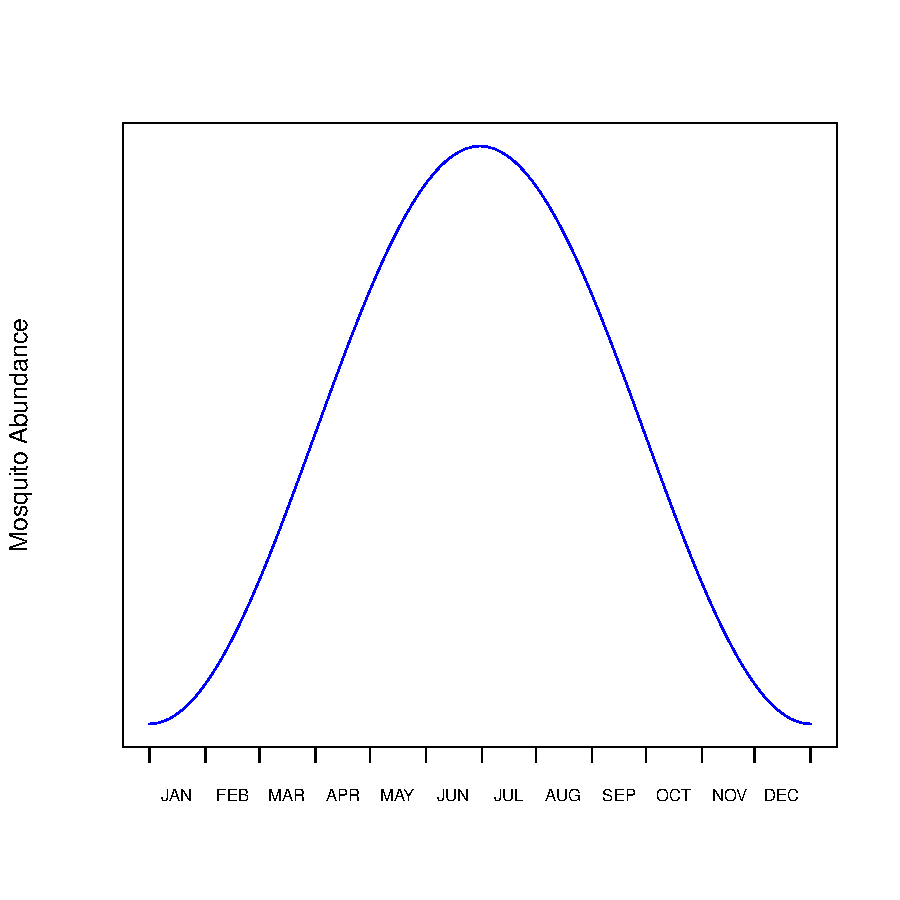
\includegraphics{moz-model-pres-plotfig1}
\end{center}
\end{figure}
% this is a not uncommon model of a seasonally varying vector population.
}

\frame{
\frametitle{But\ldots}
\begin{figure}
\begin{center}
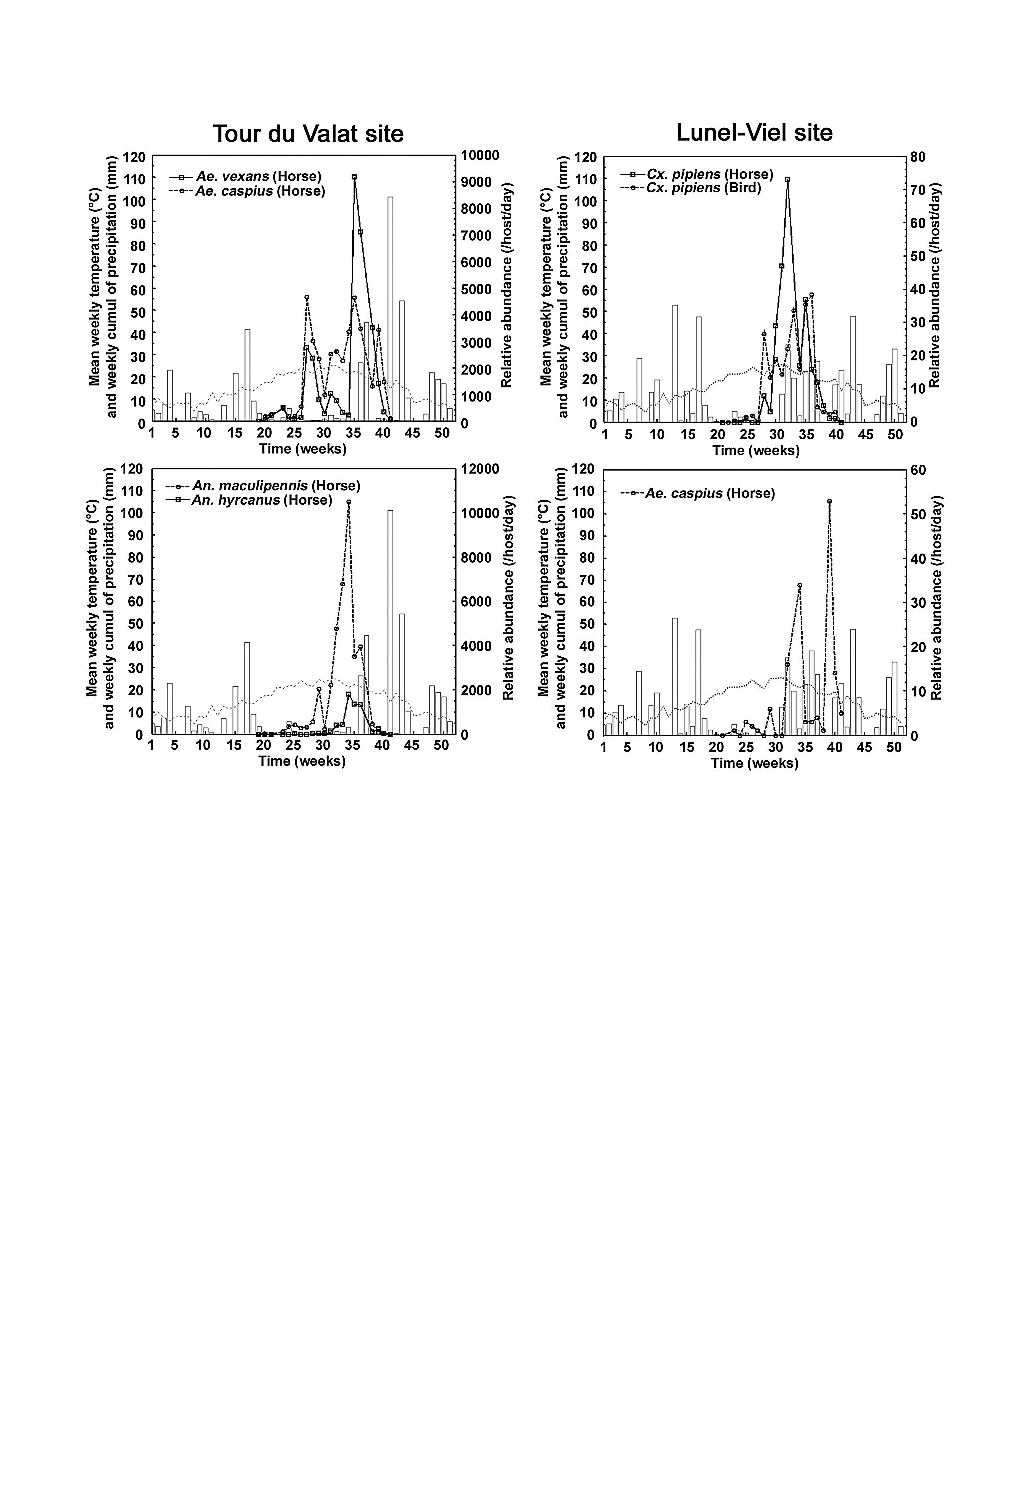
\includegraphics[width=0.9\textwidth]{insert.pdf}
\caption{Bicout et al. J. Med. Entomol. 43(5): 936-946 (2006)}
\end{center}
\end{figure}
% this is a not uncommon measurement of a seasonally varying vector population.
}

\frame{
\frametitle{So, a Disconnect.}
With

$$
M(t) = C\sin(\omega t+\theta)
$$

Impossible to match features like
\begin{itemize}
\item peak population,
\item total population over a year, and
\item turnover rate
\end{itemize}

These can be critical to predicting transmission dynamics.
% the model and the plot were noticeably different.  That doesn't always matter, but sometimes it can, and (though I don't talk about it in this short format) it definitely does for vector mediated infection.  Think about a really simple intervention: spraying insecticide to keep the mosquito population below a certain level.  If you assume the trigonometric version, you can buy the wrong amount (both too little and too much) depending on that level relative to the peak.  That's before even considering that you might have incorrectly picked the level based on a sine model.
}

\frame{
\frametitle{Do Better, But Keep It Simple}
What's good about trigonometric representation?  Simplicity:

\begin{itemize}
\item two parameters
\item no spatial features
\item ``easy'' analytical form
\end{itemize}

Possible to identify alternatives that {\em can} match salient features, but still retain these features?
% there's a lot to be said for a trignometric representation.  We get oscillation for ``free''
}

\frame{
What are those salient features?  Let's look again.
}

\frame{
\begin{figure}
\begin{center}
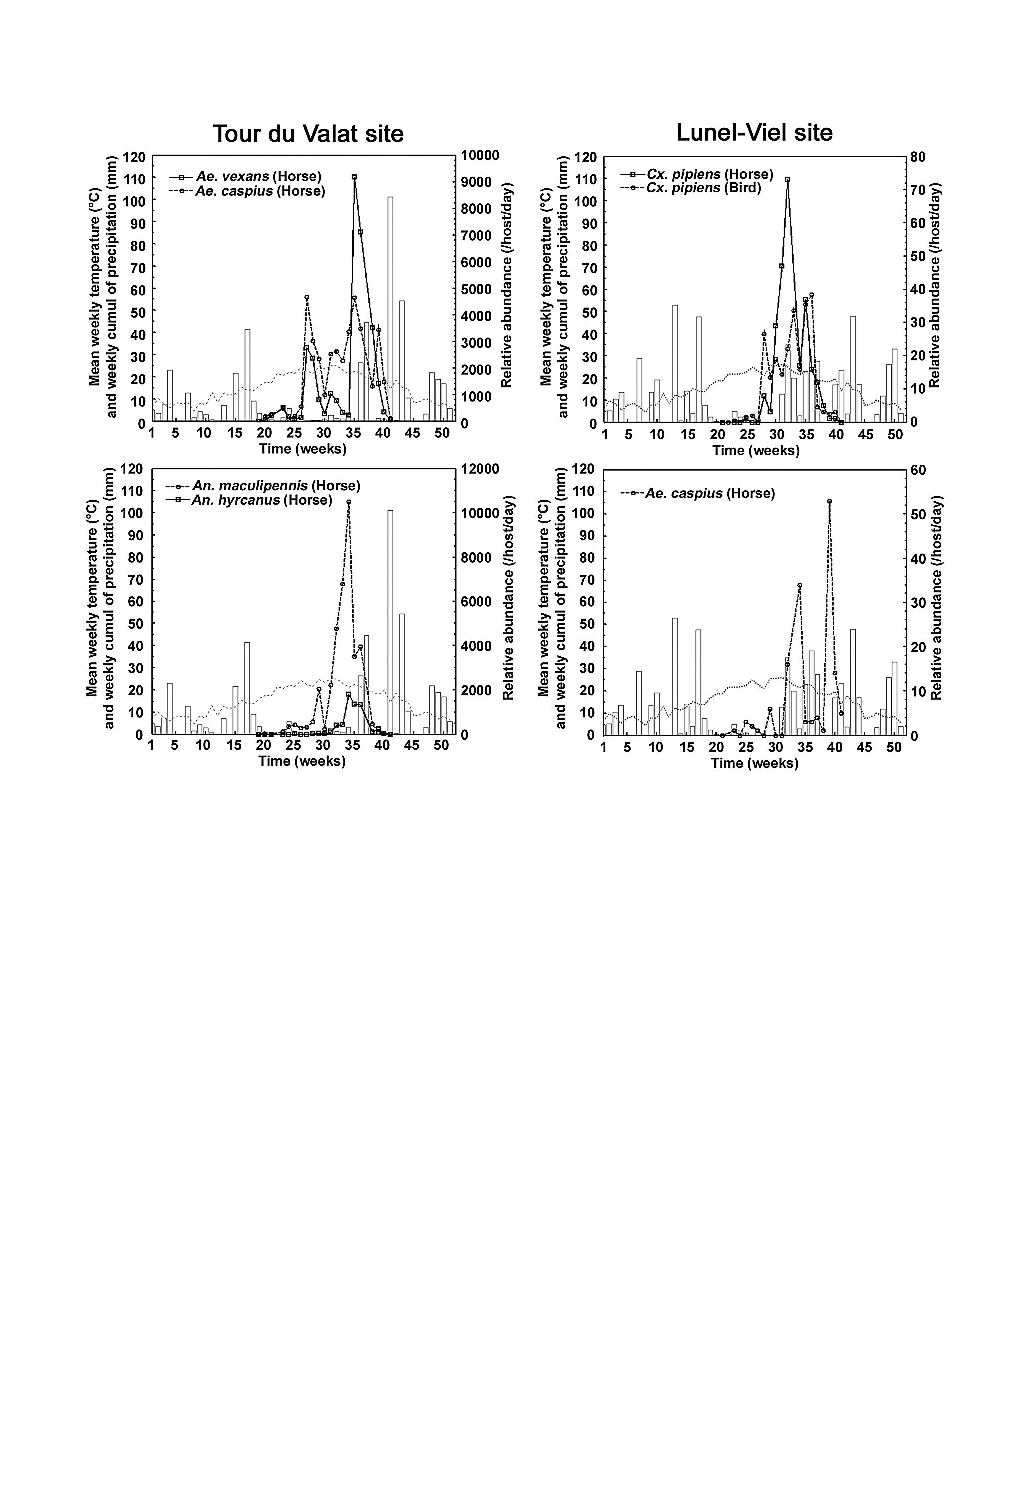
\includegraphics[width=0.8\textwidth]{insert.pdf}
\end{center}
\end{figure}
}


\frame{
\begin{itemize}
\frametitle{Salient Features}
\item every year,
\item over a relatively short duration,
\item the mosquito population rapidly increases,
\item sits at a high level of activity,
\item then rapidly declines,
\item apparently connected with resource availability \&\ environmental suitability
\end{itemize}
% aside: and if you dig around the experimental data, there are also situations where the mosquito population looks almost exactly like a trignometric function! so, ideally we want a form that has a (co)sine like form for certain parameters
}

\frame{
\frametitle{Salient Features in Trig. Representation}
\begin{itemize}
\item every year, {\bf CHECK!} \ldots {\em but not the rest of:}
\item over a relatively short duration,
\item the mosquito population rapidly increases,
\item then rapidly declines,
\item apparently connected with resource availability \&\ environmental suitability
\end{itemize}
}

\frame{
\frametitle{Getting at the Other Points}
Need:

\begin{itemize}
\item worth connecting to external force
\item ``spikey''
\item oscillatory
\end{itemize}

Can get that with repeating boundary conditions on

$$
\dot{M(t)} = E(t) - \lambda M(t)
$$

and appropriate $E(t)$.
%and also just guess that mosquitos, like many other ecological phenomena, decay exponentially when their external resource supply is removed.
}

\frame{
\frametitle{Appropriate $E(t)$}
Most of the criteria boildown to a ``spikey'' function options.  Suggestions?
\bskip
% suggestions for those?
What else would we need to ensure?
% that those functions share some features so that we're making oranges-to-oranges comparison.  This amounts to picking what features we want to match between those functions.  Extrema are common points to match, but to match M(t) extrema, we are doing so after some mathematical contortions.  I'd much prefer to put the matching constraints on E(t), while still having them correspond to an M measurement.  One easy option, and the one I've choosen to go with, is to match the integral of E over the interval.
}

\frame{
\frametitle{Alternatives I}
\begin{align*}
E(t) &= \begin{cases}
        \dfrac{\Mp}{\Dt} & t \in \Dt \\
        0 & \textrm{otherwise}
        \end{cases}\tag{Step} \\
E(\rho, t) &= \begin{cases}
        \dfrac{2\Mp}{\Dt(2-\rho)} & t \in \Dt(1-\rho) \\
        \dfrac{2\Mp}{\Dt(2-\rho)\rho}\left(1-\dfrac{2|t|}{\Dt}\right) & t \in \rho\Dt \\
        0 & \textrm{otherwise}
        \end{cases}\tag{Modified Step} \\
E(t) &= \dfrac{2\Mp}{\Dt}\sqrt{\dfrac{2}{\pi}}e^{-\dfrac{8t^2}{\Dt^2}}\tag{Approximate $\delta$}
\end{align*}
}

\frame{
\frametitle{Alternatives II}
\begin{align*}
E(t) &= \dfrac{\Mp}{\Dt}\sqrt{\dfrac{2}{\pi}}e^{-\dfrac{\sin^2 \omega t }{\omega^2\Dt^2}}\quad (\omega = \dfrac{\pi}{T})\tag{Trig. Approximate $\delta$} \\
E(t) &= \dfrac{\Mp}{T}\left(1+\cos\left(\frac{2\pi}{T} t\right)\right)\tag{Trig.} \\
E(t) &= \dfrac{(2^n n!)^2}{(2n)!}\dfrac{\Mp}{T}\cos^{2n}\left(\frac{4\pi}{T} t\right)\quad (n=\lfloor 2^{-1}\sin^{-2}\dfrac{\pi\Dt}{2T}\rfloor)\tag{Proper Trig.} \\
E(c,t) &= \dfrac{\Mp}{\Dt}\left[\dfrac{1}{1+e^{-c(t+\Dt/2)}}-\dfrac{1}{1+e^{-c(t-\Dt/2)}}\right] \tag{Double Logistic} \\
\end{align*}
}

\frame{
\frametitle{Aside: Dimensional Analysis}
Those equations have a lot of parameters, as do the resulting integral solutions.
\bskip
Fortunately, everything you learned in engineering coursework can apply here as well.
\bskip
So, how can remove the scales?
% at first glance, it seems impossible that we can get the kind of value out of dimensional analysis that we can in, say, aerodynamics.  However, there's some increasing evidence about temperature and humidity moderated vector activity / disease transmissibility / incubation times.  Some of it is switch-like, some of it appears to be a smooth transition.  We can also potentially enforce a strong control on the \Mp parameter, which is important when we carry this rescaling through to transmission dynamics
% ultimately, chose to scale by period and \Mp
% \Mp disappears un-interestingly into M, but T remains in a scale decay parameter
}

\frame{
\frametitle{Scale-free Alternatives I}
\begin{align*}
\tE{\rho,\tau} &= \begin{cases}
        \dfrac{1}{\rho} & |\tau| \le \rho/2 \\
        0 & \textrm{otherwise}
        \end{cases}\tag{Step} \\
\tE{\rho,\rho_\Delta, \tau} &= \begin{cases}
        \dfrac{2}{\rho(2-\rho_\Delta)} & \tau \in \rho(1-\rho_\Delta) \\
        \dfrac{2}{\rho(2-\rho_\Delta)\rho_\Delta}\left(1-\dfrac{2|\tau|}{\rho}\right) & \tau \in \rho\rho_\Delta \\
        0 & \textrm{otherwise}
        \end{cases}\tag{Modified Step} \\
\tE{\rho,\tau} &= \dfrac{2}{\rho}\sqrt{\dfrac{2}{\pi}}e^{-\dfrac{8}{\rho^2}\tau^2}\tag{Approximate $\delta$}
\end{align*}
}

\frame{
\frametitle{Scale-free Alternatives II}
\begin{align*}
\tE{\rho,\tau} &= \dfrac{1}{\rho}\sqrt{\dfrac{2}{\pi}}e^{-\dfrac{\sin^2 \pi \tau }{\pi^2\rho^2}}\tag{Trig. Approximate $\delta$} \\
\tEt &= \left(1+\cos{2\pi\tau}\right)\tag{Trig.} \\
\tE{\rho,\tau} &= \dfrac{(2^n n!)^2}{(2n)!}\cos^{2n}4\pi\tau\quad (n=\lfloor 2^{-1}\sin^{-2}\dfrac{\pi\rho}{2}\rfloor)\tag{Proper Trig.} \\
\tE{\tilde{c}=cT,\rho,\tau} &= \dfrac{1}{\rho}\left[\dfrac{1}{1+e^{-\tilde{c}(\tau+\rho/2)}}-\dfrac{1}{1+e^{-\tilde{c}(\tau-\rho/2)}}\right] \tag{Double Logistic} \\
\end{align*}
}

\frame{
\frametitle{The Resulting Mosquito Populations}
The analytical work to get exact $M(t)$ is\ldots tedious.  Thankfully, there are numerical integrators!
\bskip
Which gives us a window to qualify these alternatives rapidly, and then decide which to thoroughly investigate.
}


\frame{
\begin{figure}
\begin{center}
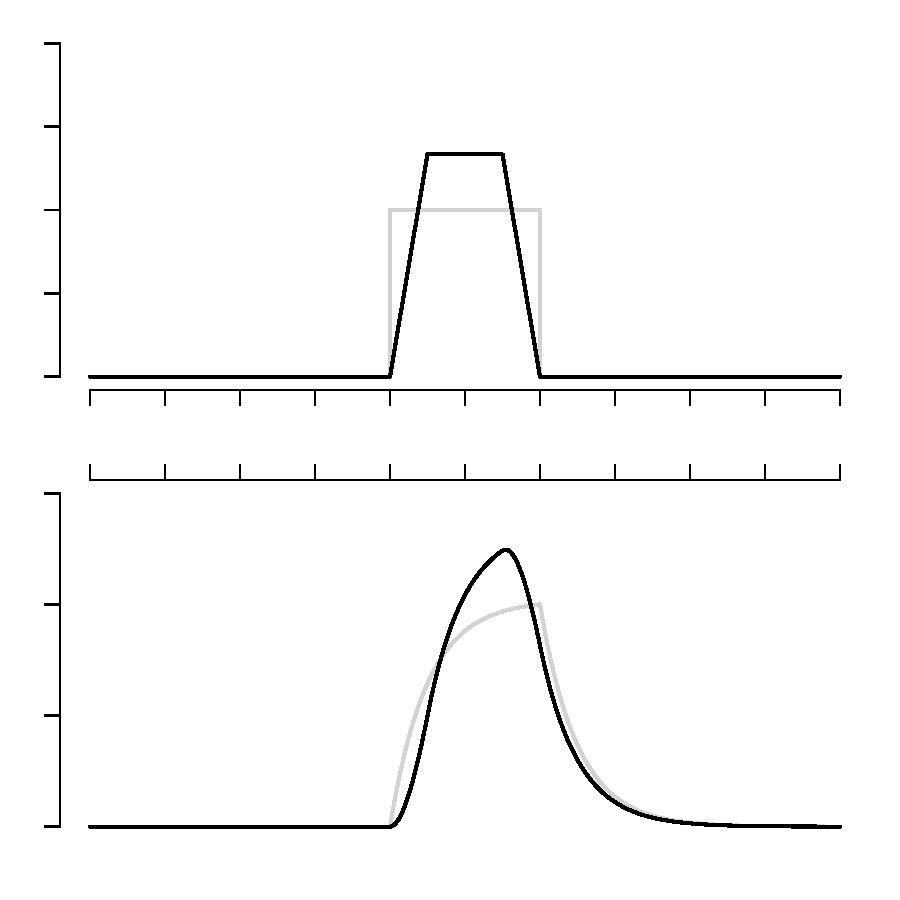
\includegraphics{moz-model-pres-pstrap}
\end{center}
\end{figure}
}

\frame{
\begin{figure}
\begin{center}
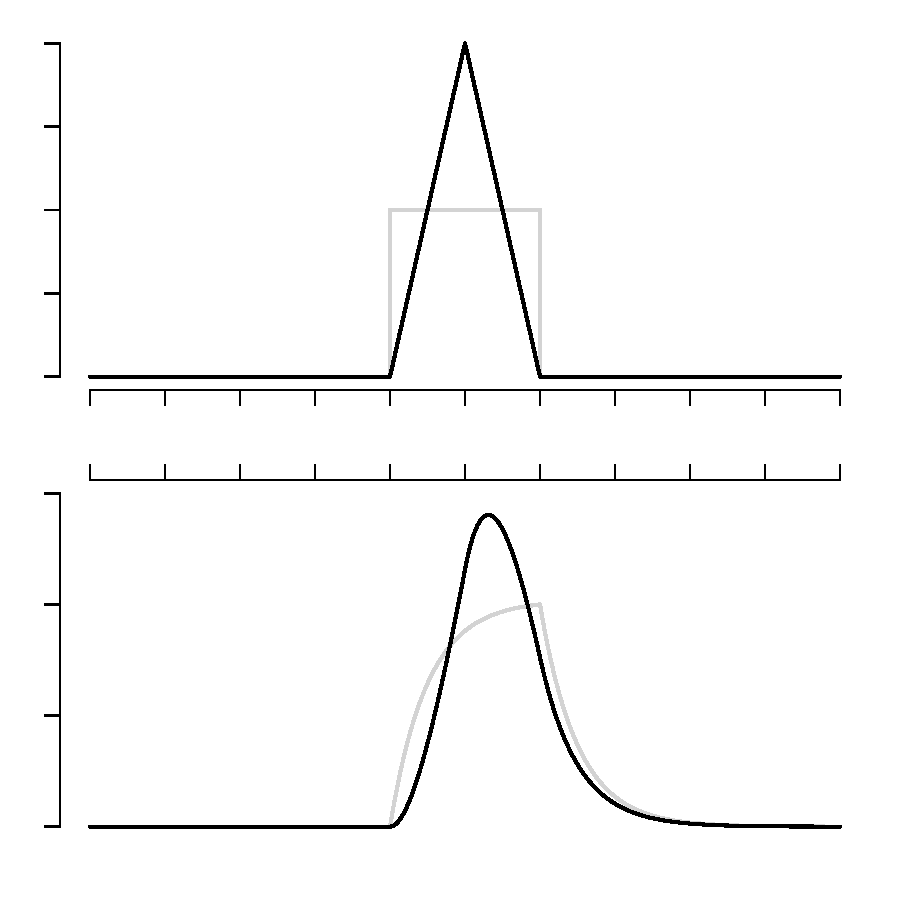
\includegraphics{moz-model-pres-pstri}
\end{center}
\end{figure}
}

\frame{
\begin{figure}
\begin{center}
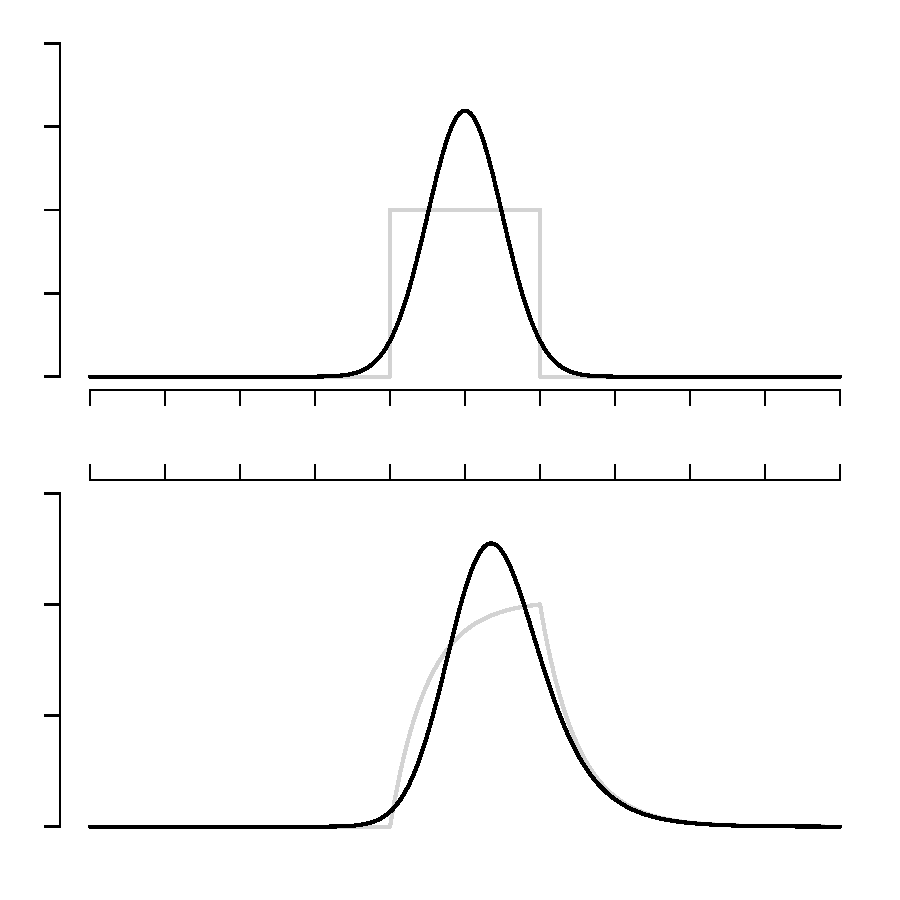
\includegraphics{moz-model-pres-psdel}
\end{center}
\end{figure}
}

\frame{
\begin{figure}
\begin{center}
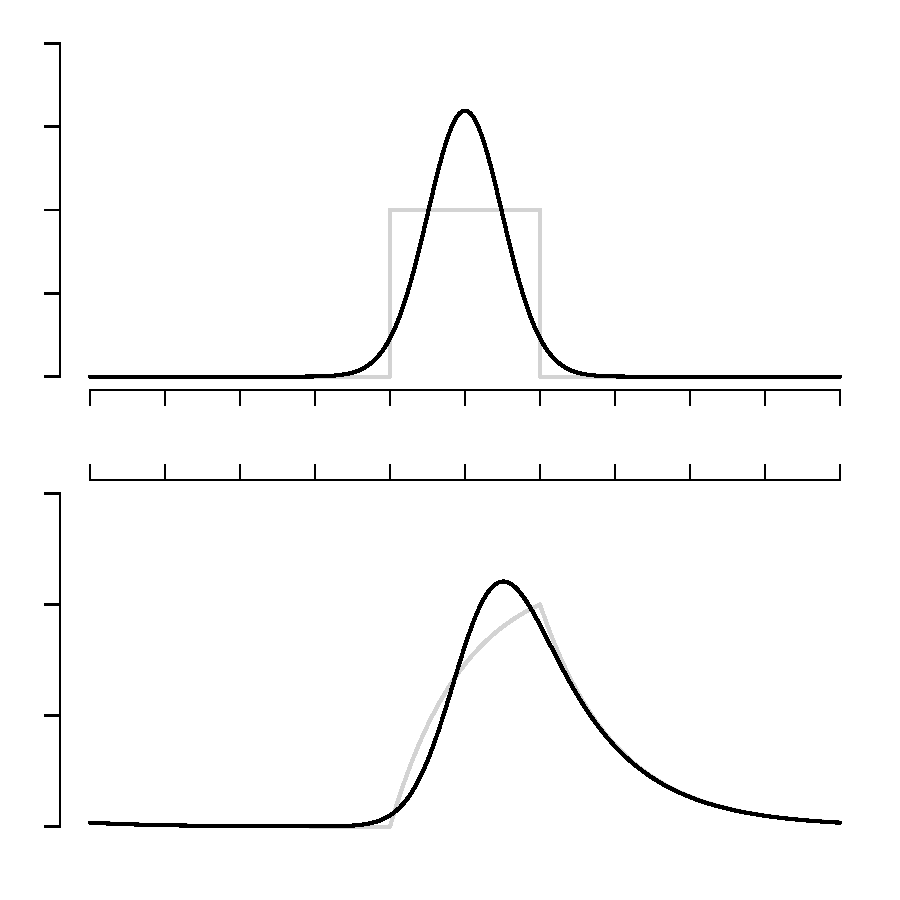
\includegraphics{moz-model-pres-psdeltrig}
\end{center}
\end{figure}
}

\frame{
\begin{figure}
\begin{center}
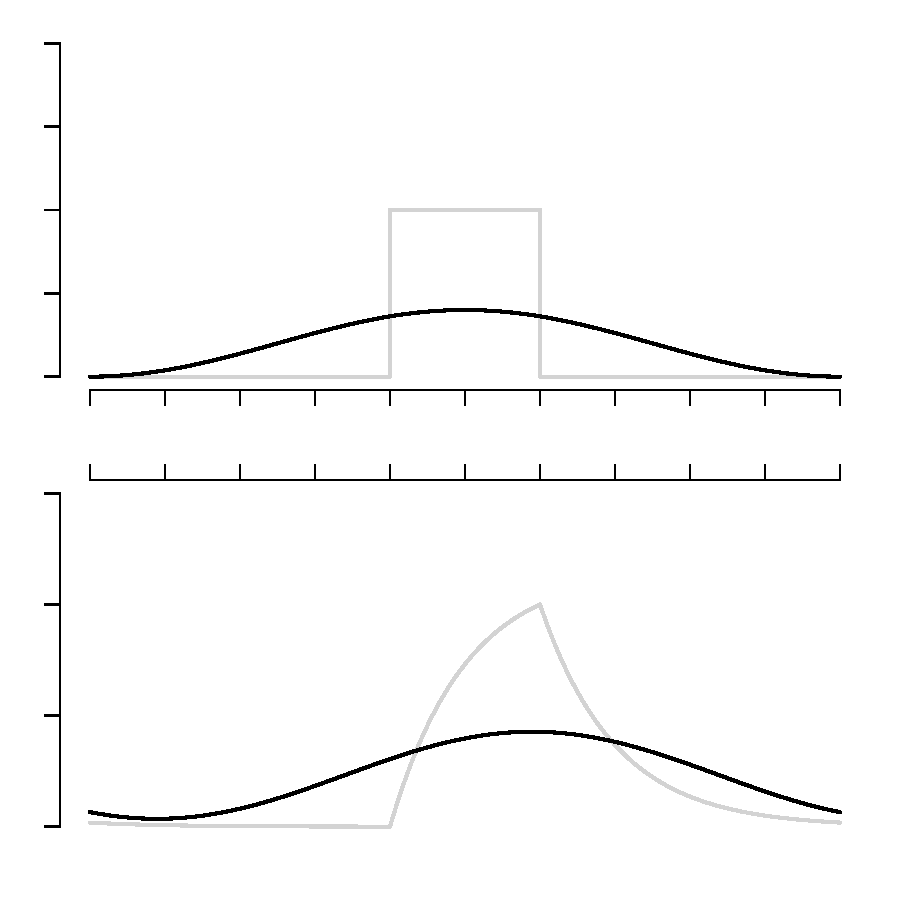
\includegraphics{moz-model-pres-pstrig}
\end{center}
\end{figure}
}

\frame{
\begin{figure}
\begin{center}
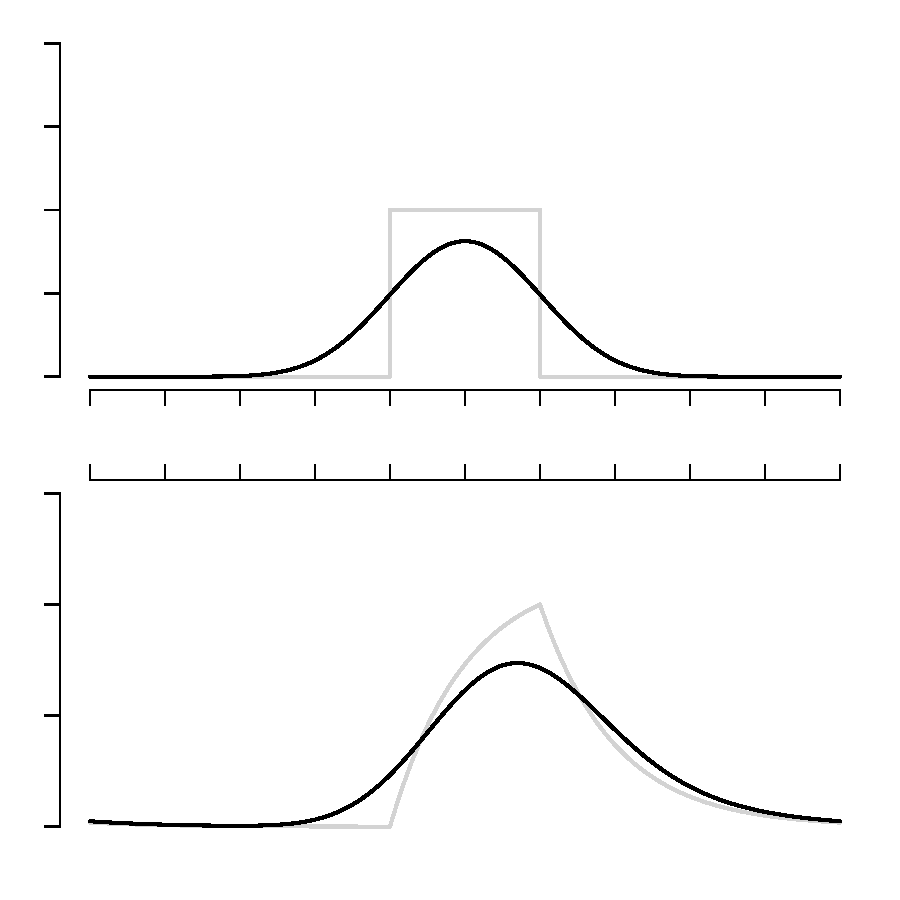
\includegraphics{moz-model-pres-pstrigprop}
\end{center}
\end{figure}
}

\frame{
\begin{figure}
\begin{center}
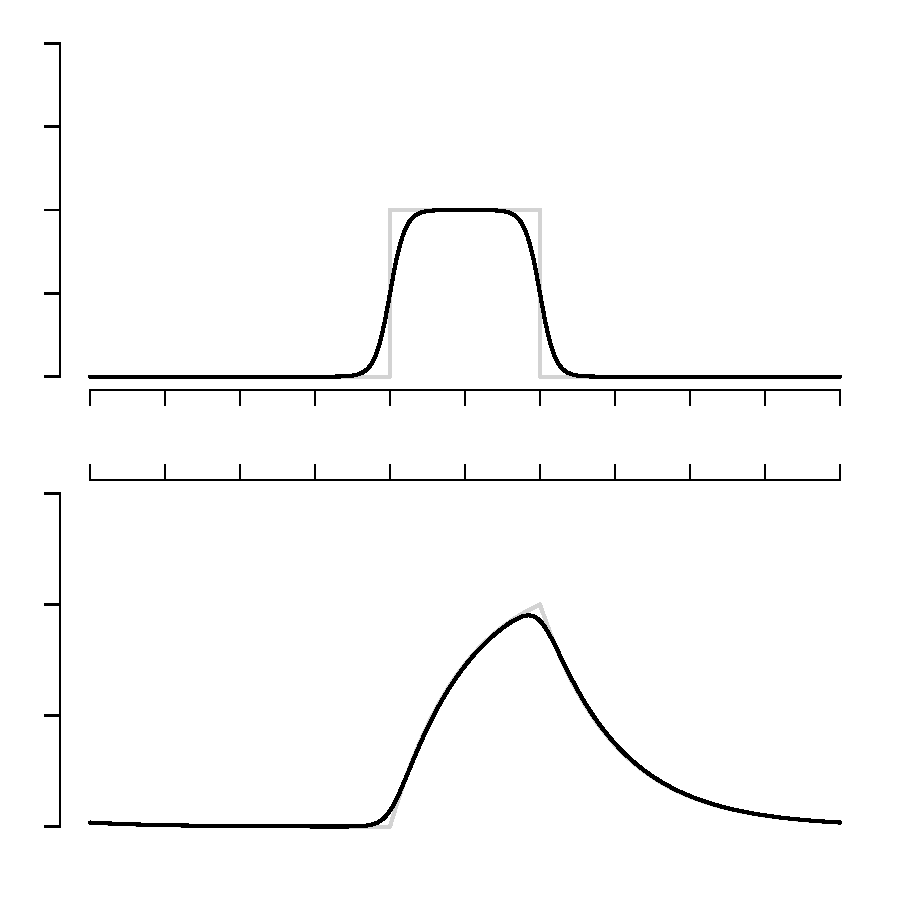
\includegraphics{moz-model-pres-pslog}
\end{center}
\end{figure}
}

\frame{
\frametitle{Thoughts?}
What do {\em you} think about the options?
%I'm inclined to say they are all the same!
}

\frame{
\begin{figure}
\begin{center}
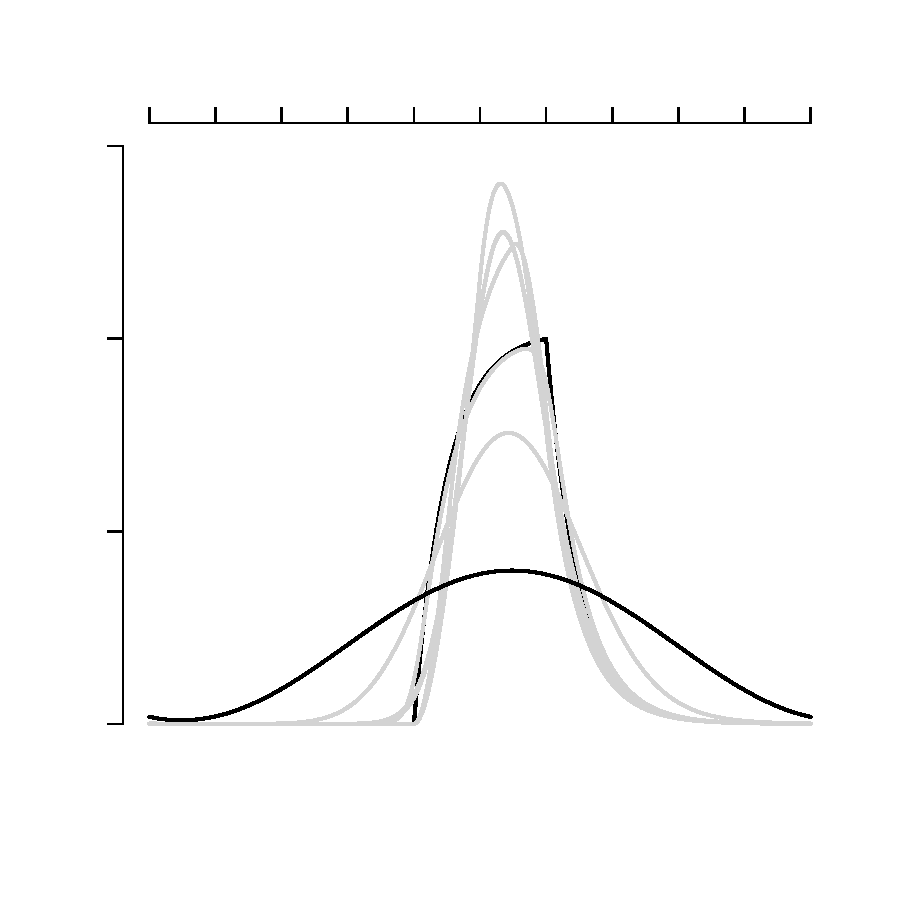
\includegraphics{moz-model-pres-psmix}
\end{center}
\end{figure}
}


\frame{
\frametitle{Back To Oversimplification Question}
Are these alternatives still too simple?
\bskip
They are all built assuming a stable driver, which is inaccurate.
\bskip
But: this framework presents an easy way to consider $E(t)$ changes as perturbations.
% and rapidly compare across E(t) options
%That is, given the stable solution at the start of a period, how do changes to the driver in that period transform the end-of-period outcome?
% and thus the next period, and so on.  If driver changes are mostly damped, then it makes a lot of sense to talk about an average annual outcome and then perturb it given a short history / some forecasting.  This makes both near and long prediction (with confidence intervals) a much more tractable task.  It also provides a lot of power when talking about structural shifts (e.g., more average rainfall / longer suitable temperature ranges for foreseeable future)
% this is one of the next steps in this particular project
}

\frame{
\frametitle{So What?}
What does this basic analysis give us?
\begin{itemize}
\item rough boundaries as input to other models,
%A complete picture of a disease has several interacting parts.  This particular work is associated with Japanese Encephalitis Virus, and how it moves between wildlife, livestock (pigs), and humans.  This analytical work maps out the interesting jigsaw borders for mosquito populations, which we in turn use with an agent-based model of mosquito, livestock, and human interaction.  That model is in turn fit with an Approximate Bayesian Computation tool
\item where more complex approaches are needed (agent-based, spatially explicity, {\em etc}.)
%For example, this model de-couples mosquito reproduction from their population.  There are ecological ranges where this is fine, but if you wanted to consider an optimal control style real-time intervention, you'd need to consider what the population looks like at very low levels and its amplification rate.  I've done this sort of analysis for neutron transport in reactor design -- shooting from the hip, that kind of mosquito control is a lot harder problem
\item a component connectable to other models
\end{itemize}
}

\frame{
\frametitle{Seque: Need ``New'' Habits and Tools}
New challenges to getting science done:
\begin{itemize}
\item lashing together methods from different fields,
\item getting genuine peer-review, and
\item the purely mechanical handling of different people simultaneously working on the same ``thing''
\end{itemize}

How can we address these issues?
% The general arrow of scientific work has been towards increased specialization and collaboration, and to increasingly digitally-based components.
%.  The final specialist work product can be very intimidating to collaborators with other specialities, which can make a collaboration's skeptical review of their combined product difficult. That's on top of the pure mechanics of handling multiple people modifying the same ``thing''.
% I come from a background where all collaborators are responsible for the entire product, not just their narrowly focused piece
}

\frame{
\frametitle{Solutions from Software Industry?}
What tools and habits can we adopt from this field?
\bskip
What risks are associated with that?
\bskip
What's still missing?
}

\frame{
\frametitle{The Good}
\begin{itemize}
\item version control systems,
\item collaborative tools on top of those,
\item preference for code documentation leading to
\begin{itemize}
\item bite-sized parts,
\item modularity,
\item re-usability, and
\item verifiability (a/k/a unit testing)
\end{itemize}
\item open availability of all source,
\item combines with version control to provide complete history of work product
\end{itemize}
}

\frame{
\frametitle{The Bad}
\begin{itemize}
\item openness can make for opportunity to be ``scooped'',
\item can focus more on process than product,
\item learning curve for most scientists
\end{itemize}
}

\frame{
\frametitle{The Ugly}
\begin{itemize}
\item university contracts' intellectual property clauses,
\item academic institutions don't ``get'' these tools,
\item community adoption?
\end{itemize}
}

\definecolor{TrWhite}{RGB}{200,200,200}
\usebackgroundtemplate{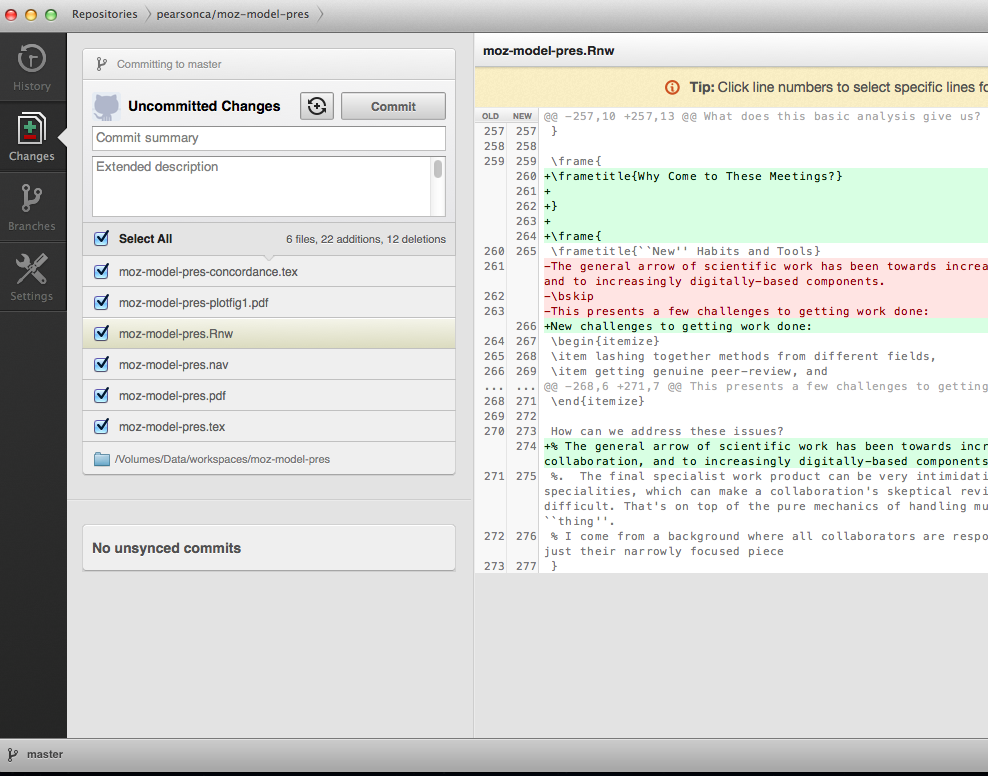
\includegraphics[width=\paperwidth,height=\paperheight]{githubbg.png}}
\setbeamercolor{block body}{bg=white}
\setbeamercolor{block title}{bg=lightgray}
\frame{
\begin{block}{Why bring this up?}
It's a little bit advocacy, and I built this presentation using this work model.
\bskip
\href{http://github.com/pearsonca/moz-model-pres}{http://github.com/pearsonca/moz-model-pres}
\end{block}
}
\usebackgroundtemplate{}

\frame{
\frametitle{Why Come to These Meetings?}

}

\end{document}
